\chapter[2022 September]{September 2022}

\section[2022/09/07]{Wednesday, 07 September 2022}

\subsection{First principles neural network}

The aim of this session is to elucidate the recent progress made on the first principles gesture recognition system.

The success of the open hand/fist classifier led to the hypothesis that the virtual object could be adequately controlled by combining the outputs of multiple single gesture/orientation classifiers to build up a model of the current form of the user's hand or gesture. Thus, three classifiers were implemented using Tensorflow - the one specified above that differentiaties between an open hand or closed fist, a classifier that detects whether the palm, back or side of the hand is facing towards the camera and finally if the hand is pointing up, left or right relative to the camera frame - improved upon from an earlier experiment by means of data augmentation. A number of training images were taken, and a neural network modified to learn each of these features. The experiment was a success and saw over 1.0 accuracy for both the open hand/fist classifier and palm/side/back classifier. The direction classifier fared worse with only a 96\% accuracy on the test data set - but it is hypothesized that a large amount of input training data could rectify this. Having acquired the model weights using Tensorflow the goal of moving these implementations to a first principles neural network was undertaken. \\

The neural network built earlier in the year from first principles needed several modifications to achieve the same output as the Tensorflow models utilizing the same architecture. This including changing the activation function from the sigmoid function to the relu function, changing the order and output of both the convolution and maxpooling layer to the same order as the Tensorflow model, changing the Convolution layer's mathematics to allow for multiple colour channels and switching certain operations from laborious for loops to more efficient vectorization solutions - for example, the relu function was changed from an if statement returning 0 if the input value was below 0 and the value otherwise to a matrix multiplication between the entire output matrix and a same-sized matrix of ones and zeroes representing if the value at that particular position is greater than zero or not. This vastly sped up computation. The core of the convolution algorithm is still done with scipy's signal.correlate2d function as the first principles method was just too slow for meaningful inference time. Discussion of this design choice will form part of the final report. In fact, a number of components of the first principles network still need to be vectorized and optimized if real-time gesture recognition is to be performed because the current speed of each inference is 0.3 seconds - only netting a 3 or 4 frames per second output.\\

These three first principles classifiers were then combined with a slightly modified OpenGL cube program to form a working prototype of the final implementation that allows a user to move their hand close to the cube, close their hand around it and then move the cube across the image frame. Rotating the cube and interacting with the environment around the user is still an ongoing task at the time of writing.

\begin{figure}[h]
    \centering
    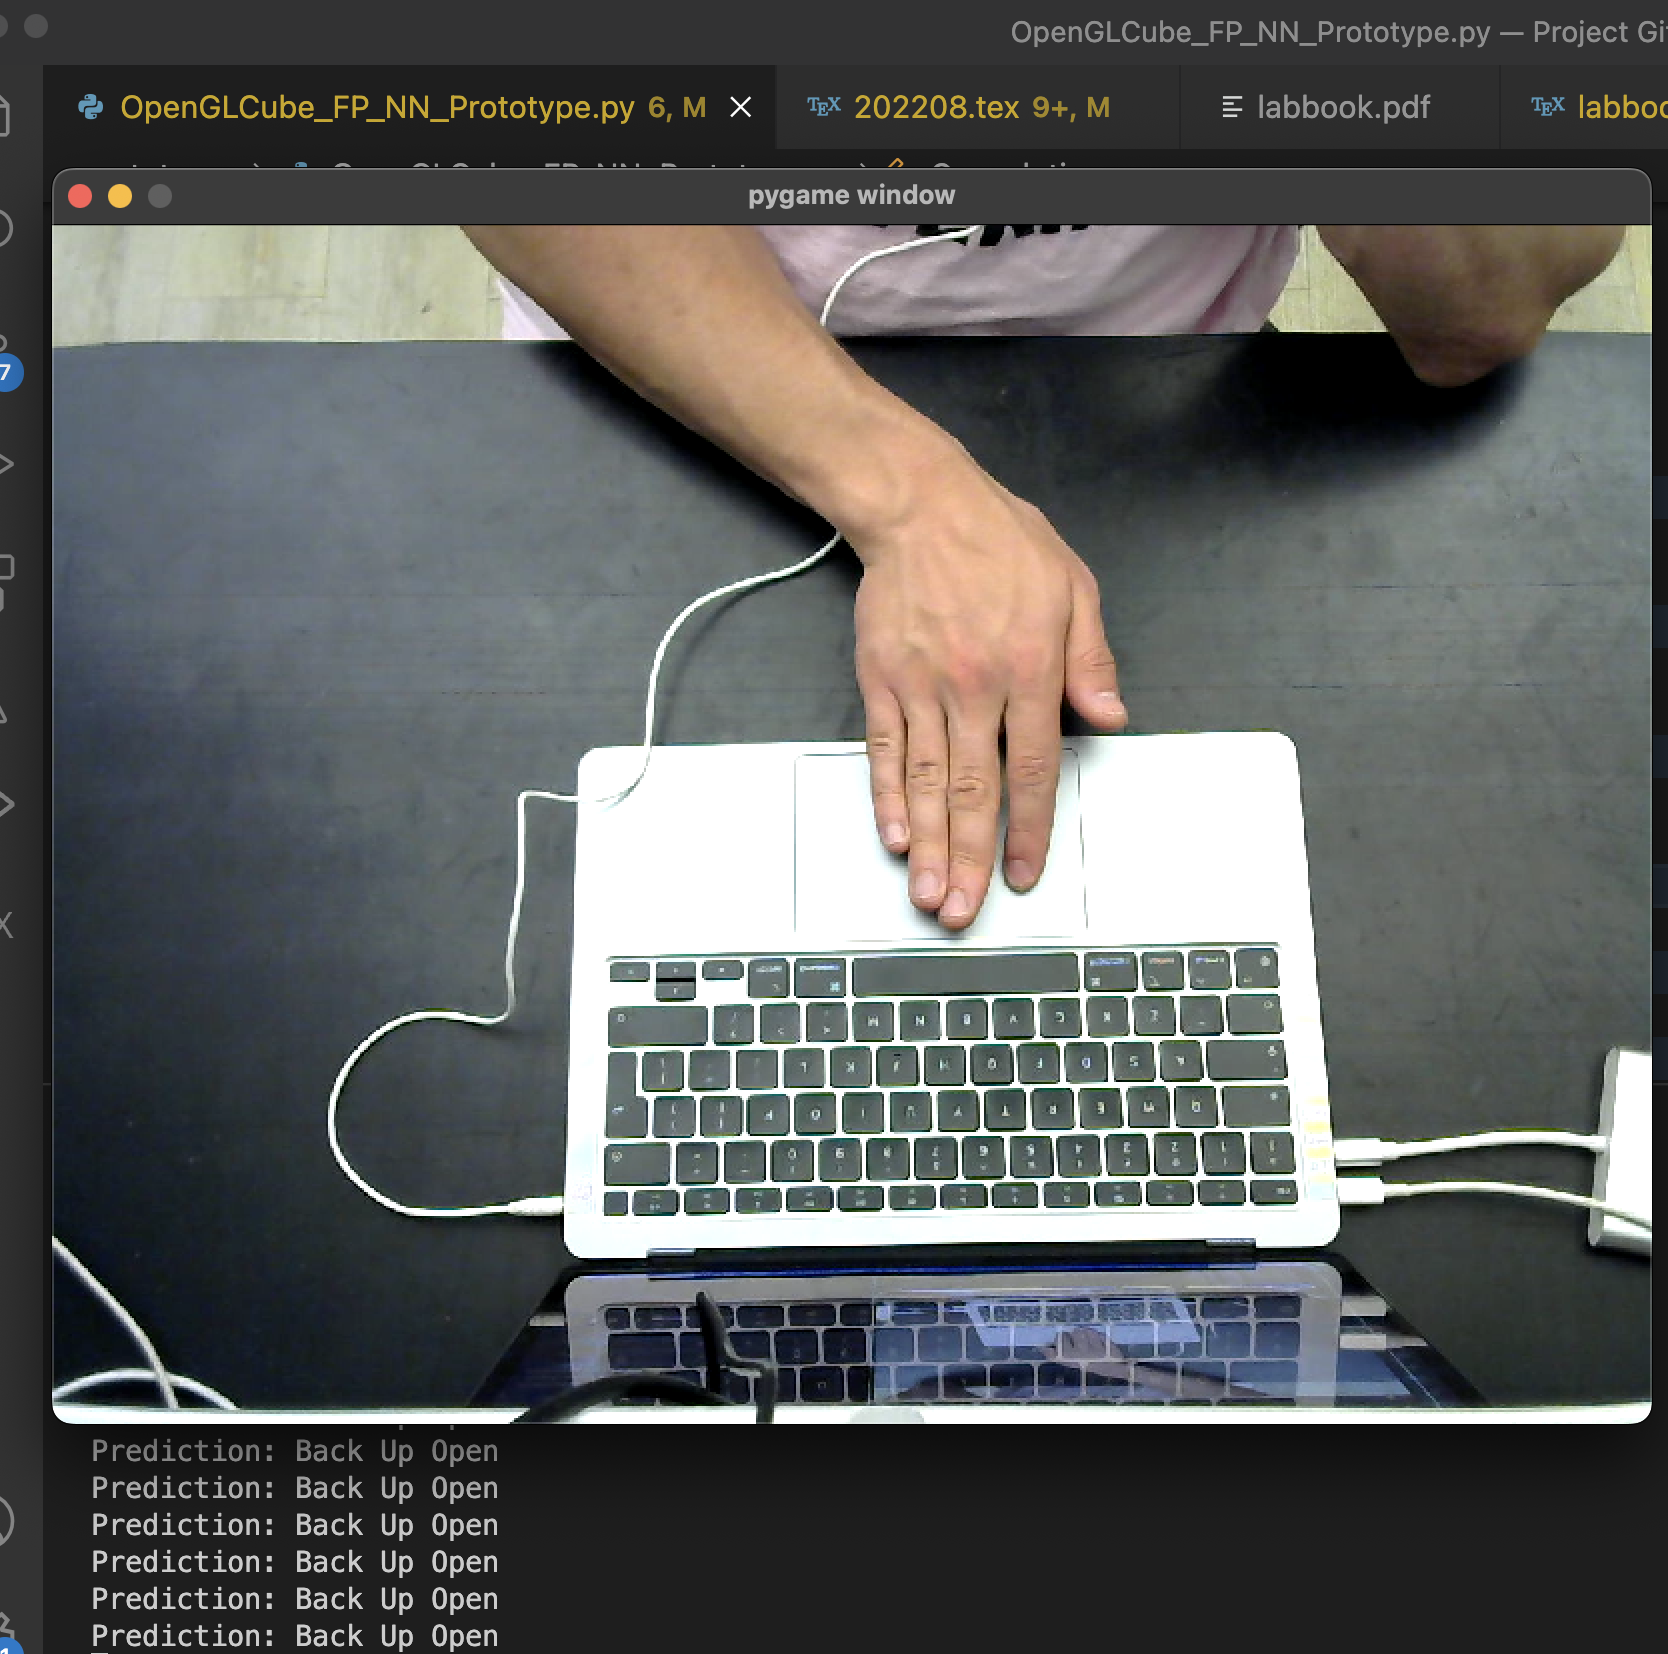
\includegraphics[width=0.7\linewidth]{figures/OpenGLCube_FP_NN_Prototype.png}
    \caption{Output of first principles gesture classifier}
    \label{fig:OpenGLCube_FP_NN_Prototype}
\end{figure}

\section[2022/09/09]{Friday, 09 September 2022}

\subsection{Kinect side-on hand tracking}

The aim of this session is to modify the hand tracking algorithm to work from a side view with the Microsoft Kinect sensor. 

Although the use of the overhead camera view is useful for gesture recognition, it is challenging to reconcile the coordinate system from a topdown camera and a camera facing the scene from the side. The Microsoft Kinect camera and depth sensor is going to be placed on the side of the user pointing at the desk because this is the view that is most desirable for the creation of the illusion of augmented reality - being able to reach into the scene in front of you and manipulate virtual objects there. However, the hand tracking algorithm was optimized for a topdown view and so needs to be modified in order to track the hand properly through the camera frame.

To this end, an axes detection algorithm was introduced which identifies which edge of the image - top, bottom, left or right, and has the most skin-coloured pixels along it and thus represents the side of the image that the user's hand and arm is entering from. From this information, the largest concentration of skin-coloured pixels closest to the opposite edge of the image can be found and this results in the hand being identified and tracked in the image. Additionally, the size of the extracted image around the hand is modified based on which edge it is closest to so that the full hand and wrist is extracted and sent on the convolutional neural network for further gesture recognition processing. The result is that the hand can be tracked accurately throughout the frame no matter which angle the user enters the frame from and thus the system is even more robust than the topdown hand tracking implementation. The output of the system can be seen in \FigRef{fig:kinect_side_hand_tracking}.

\begin{figure}[h]
    \centering
    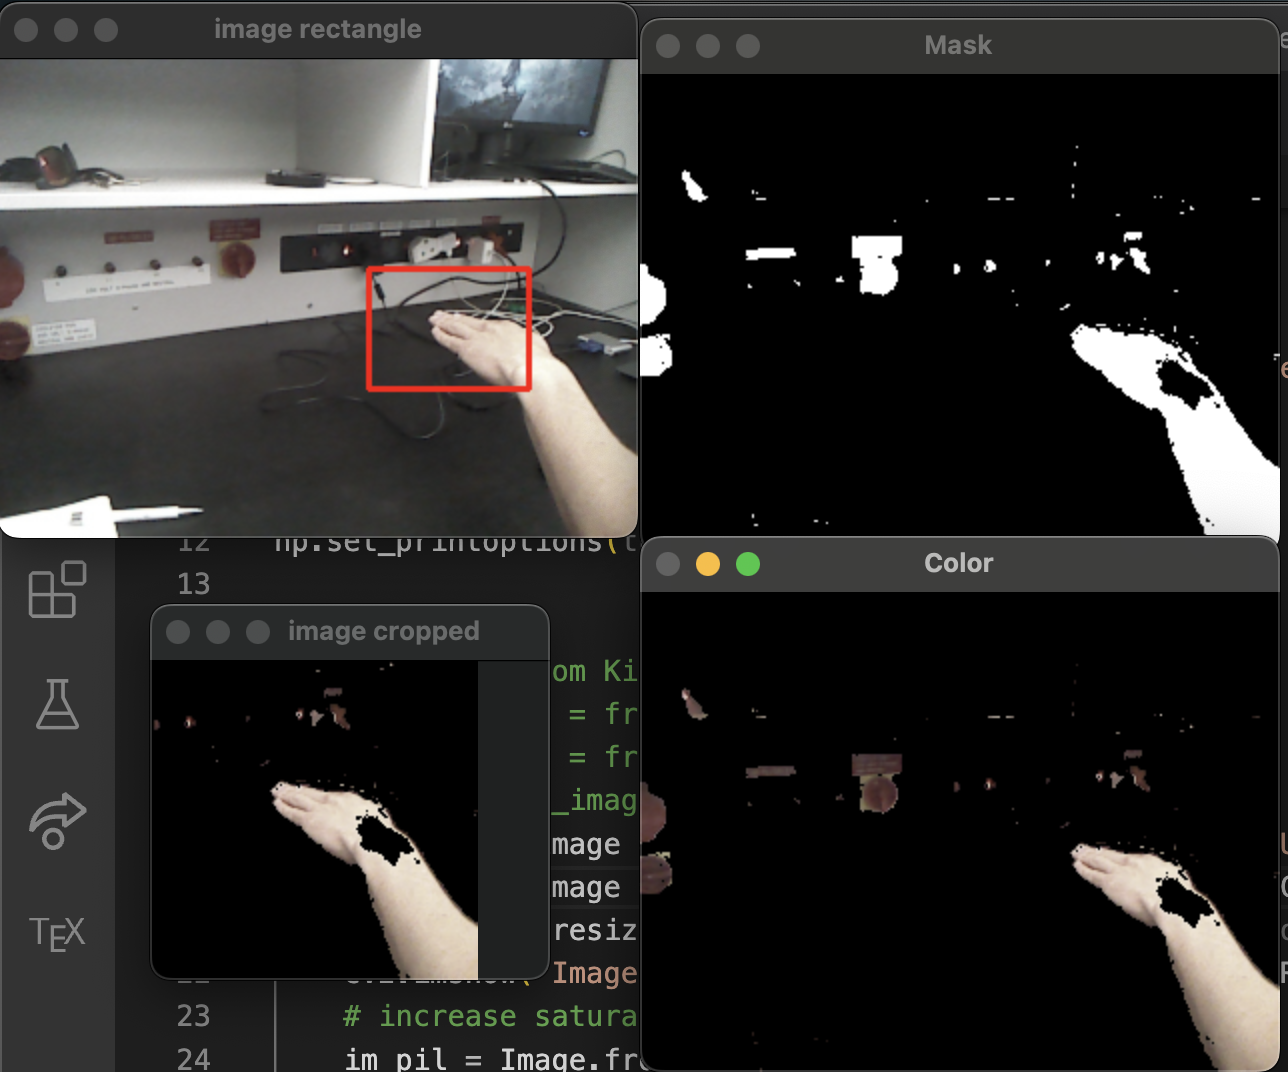
\includegraphics[width=0.7\linewidth]{figures/kinect_side_hand_tracking.png}
    \caption{Output of the side-on Kinect hand tracking}
    \label{fig:kinect_side_hand_tracking}
\end{figure}

\section[2022/09/12]{Monday, 12 September 2022}

\subsection{Speeding up first-principles neural network}

In the aid of speeding up the processing of the neural network operations, research was done these past few days on using ctypes or Cython to integrate C code with the Python first principles neural network implementation to speed up operations. Specifically, the use of cytpes to replace the Maxpooling operation was attempted and a Maxpooling implementation in C written. However, problems were encountered when trying to pass a three-dimensional matrix to the C function as the input to the maxpooling algorithm. Work on fixing that integration using pointers and static typing is still ongoing however a more elementary change was introduced to speed up computations. This took the form of reducing the image size the webcam image is resized down to before being passed into the gesture classifier neural networks. Previously the image was resized to 320 x 240 pixels and then processing would take place. This resulted in a large execution runtime for the maxpooling operation. However, after resizing the input image down to just 80 x 60 pixels, the accuracy of the gesture classifiers largely remained the same but the execution time went down from around half a second to only 0.04 seconds as shown in \FigRef{fig:smaller_image_prediction_time}. This is a massive speedup and is highly desirable considering gesture accuracy largely stayed constant. Further testing on just how small the image can be made before significant accuracy is lost will be necessary to further speed up the system.

\begin{figure}[h]
    \centering
    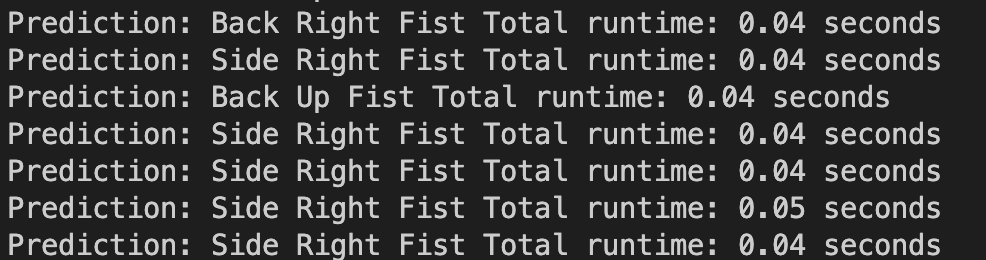
\includegraphics[width=0.7\linewidth]{figures/smaller_image_prediction_time.png}
    \caption{Output of the OpenGL First principles neural network gesture classifier prototype}
    \label{fig:smaller_image_prediction_time}
\end{figure}

\section[2022/09/22]{Thursday, 22 September 2022}

\subsection{Integrated prototype}

Recent changes to the first principles neural network include scaling down the size of the input image to the neural networks in order to increase the speed of inference as well as modifying the hand detection algorithm so that a boolean is returned that represents whether a certain threshold of masked pixels has been detected - whether a hand is present in the frame or not. This can be used later in the algorithmic pipeline in order to keep the cube static and not to run inference on an empty frame. \\

Three different classifiers are implemented in the first principles integrated prototype and these are the open/closed hand classifier, downwards-facing, side-facing or upwards-facing classifier as well as the forwards-pointing, left-pointing and downwards-pointing classifier. The results of these classifiers are experimentally used to rotate the cube in various manners consistent with how a real-world cube would behave when subjected to the hand motions recognized by the classifiers. This is visible in \FigRef{fig:integrated_prototpe_1} where the hand is pointing upwards and has rotated the cube in the relevant direction.

\begin{figure}[h]
    \centering
    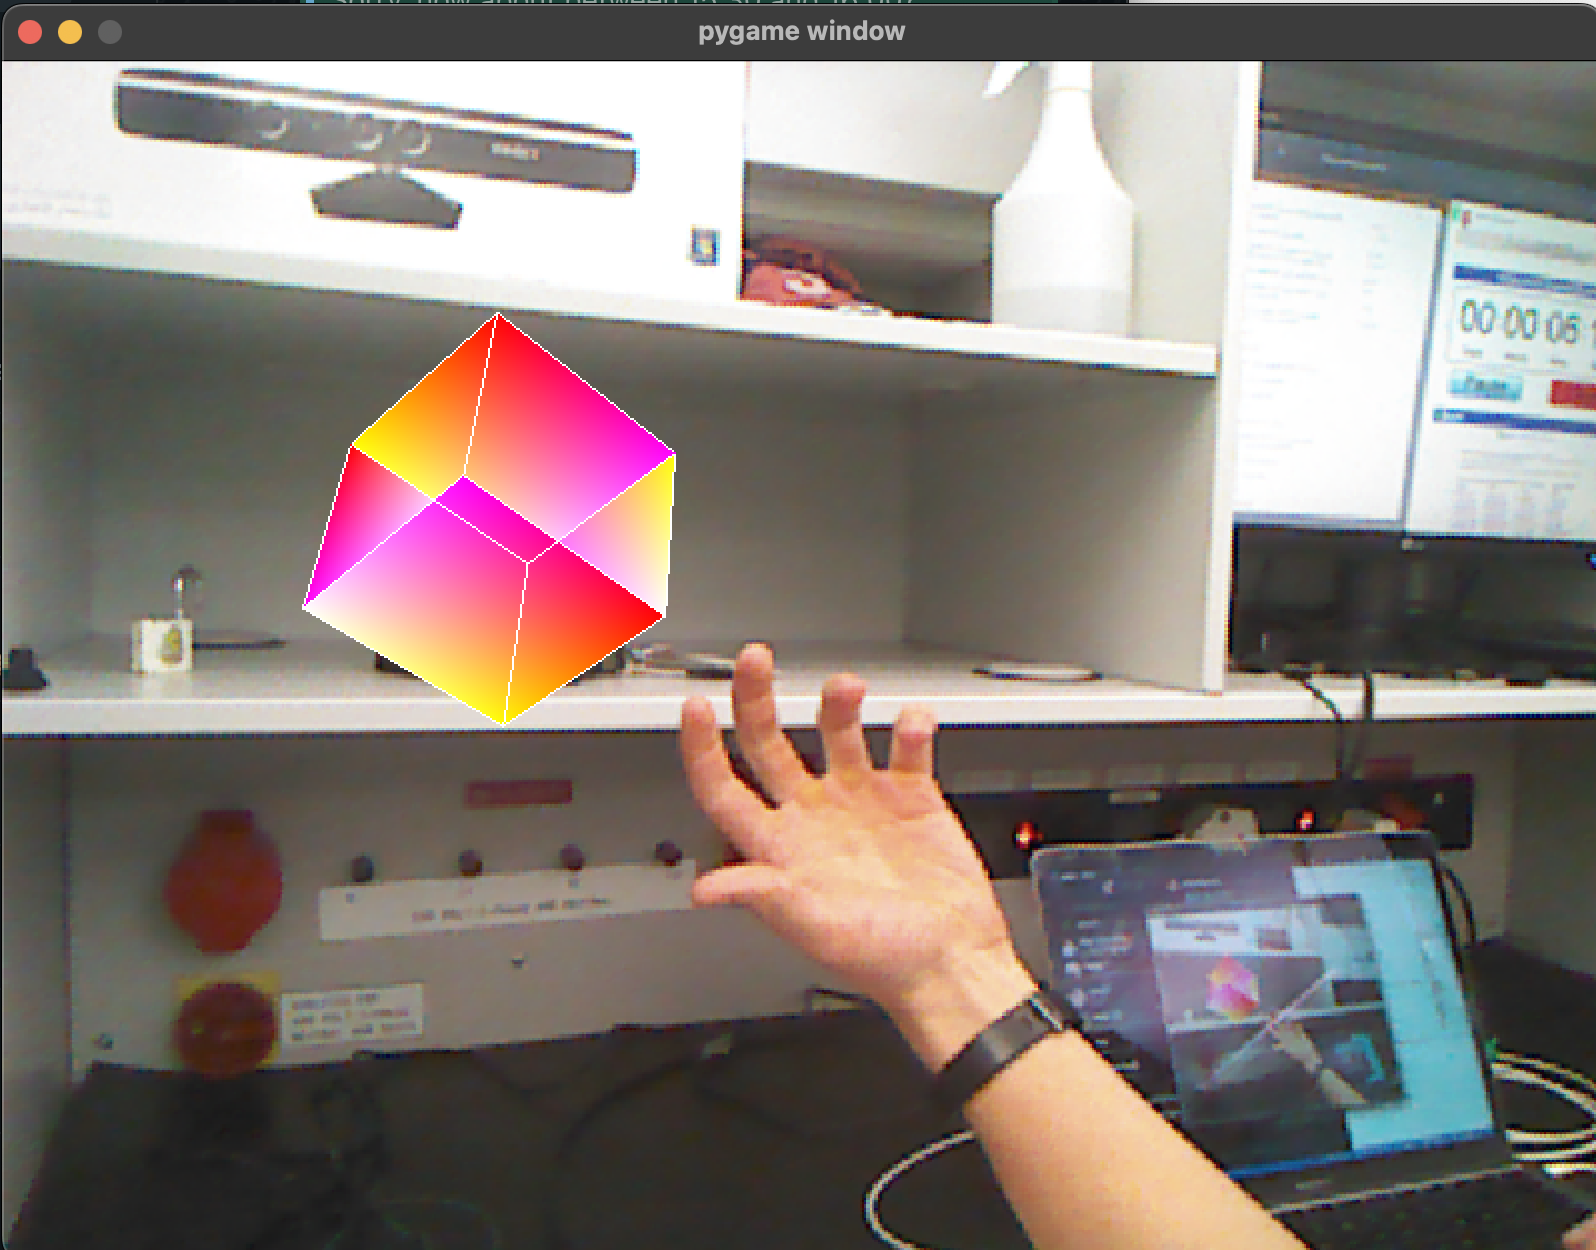
\includegraphics[width=0.7\linewidth]{figures/integrated_prototpe_1.png}
    \caption{Output of the integrated prototype cube rotation}
    \label{fig:integrated_prototpe_1}
\end{figure}

As mentioned previously, the input image is scaled down to 80x60 in the hand segmentation step and this results in much faster execution time for the three gesture classifiers. Specifically, all three classifiers finish their inference in an average of 0.0834 seconds. This is visible in \FigRef{fig:integrated_nn_speed} and results in an average frame rate of 12fps. This is half of the required frame rate specified in the project proposal but is predicted to be easily increased by experimentally reducing the size of the neural networks and changing hyperparameters while retaining the current accuracy, which is good and visible in \FigRef{fig:tf_directions_accuracy} to \FigRef{fig:tf_open_fist_accuracy}. The size of the datasets used for these classifiers was 270, 420 and 480 items large respectively. Increasing the size of these datasets and thus the accuracy of the networks and their robustness to noise and incorrect predictions is an ongoing task and will be given particular consideration for the remainder of today's session.

\begin{figure}[h]
    \centering
    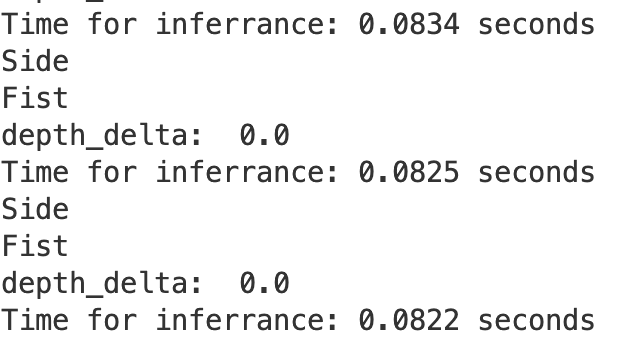
\includegraphics[width=0.4\linewidth]{figures/integrated_nn_speed.png}
    \caption{Timers showing the time taken to perform inference on an image for all three classifiers}
    \label{fig:integrated_nn_speed}
\end{figure}

\begin{figure}[h]
    \centering
    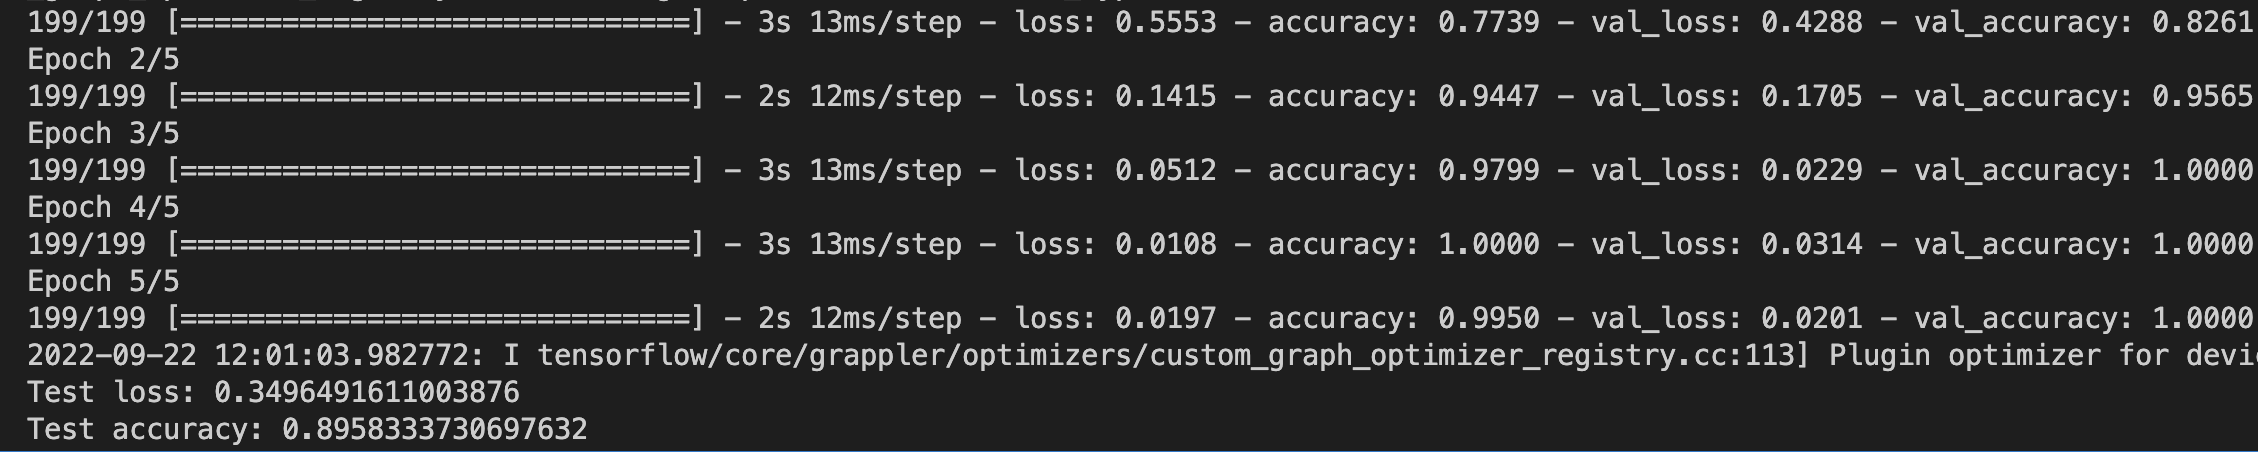
\includegraphics[width=0.7\linewidth]{figures/tf_directions_accuracy.png}
    \caption{Accuracy of Tensorflow gesture directions classifier on a 270-item large dataset }
    \label{fig:tf_directions_accuracy}
\end{figure}

\begin{figure}[h]
    \centering
    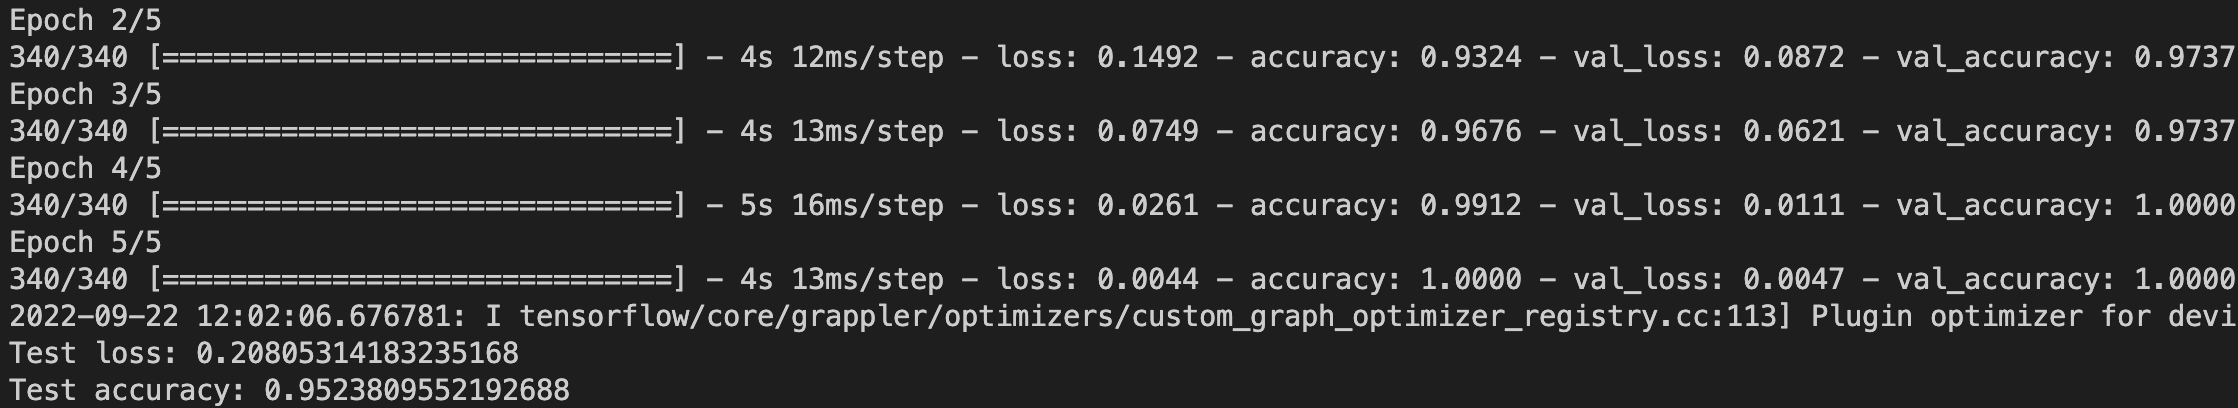
\includegraphics[width=0.7\linewidth]{figures/tf_side_down_up_accuracy.png}
    \caption{Accuracy of Tensorflow gesture down, side, upwards facing classifier on a 420-item large dataset }
    \label{fig:tf_side_down_up_accuracy}
\end{figure}

\begin{figure}[h]
    \centering
    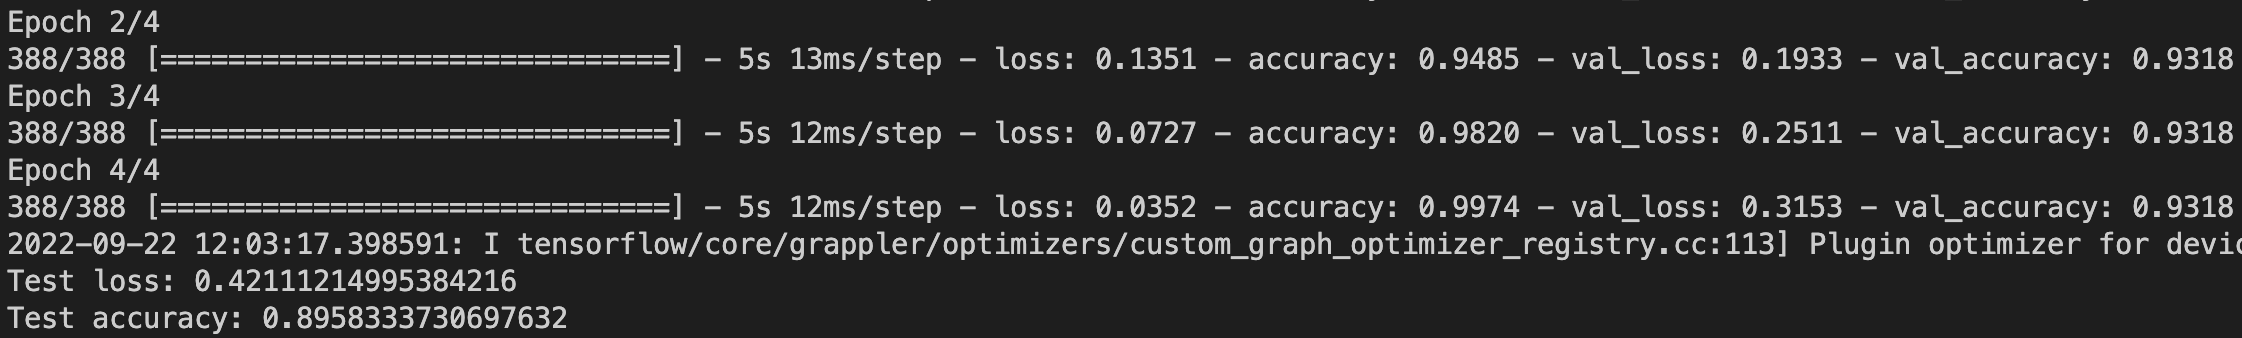
\includegraphics[width=0.7\linewidth]{figures/tf_open_fist_accuracy.png}
    \caption{Accuracy of Tensorflow gesture open/closed fist classifier on a 480-item large dataset }
    \label{fig:tf_open_fist_accuracy}
\end{figure}